\section{Example}
The approach to data-race detection in this paper is presented in a very simple example.
Consider the task-parallel program in \figref{fig:example}.
The language used is defined in this paper with a formal semantics to facilitate proofs but has a direct expression in most task parallel languages.
For example, \figref{fig:example-hj} is the equivalent program in the Habanero Java language.

For \figref{fig:example}, execution begins with the procedure \texttt{m}.
The variable \texttt{g} is global.
The \textbf{post}-statement creates a new asynchronous task running procedure \texttt{p} passing 0 for its parameter.
The task handled is stored in the region $r$, also global, and when that task completes and joins with its parent \texttt{m}, it runs the $\lambda$-expression as a return value handler.
In this case, that handler is the no-op \texttt{skip}.

The \textbf{isolated}-statement runs the statements in its scope in mutual exclusion to other \textbf{isolated}-statements.
The \textbf{await}-statement joins all tasks in region \texttt{r} with the task that issued the await.
The issuer may join with a task in the region if that task is at its \textbf{return}-statement.
The expression in the return statement is evaluated at the join and the value is passed to the return value handler in the parent context.
The parent blocks at the \textbf{await}-statement until it has joined with all tasks in the indicated region.

The program in \figref{fig:example} has a schedule dependent data race.
If the scheduler runs the \textbf{isolated}-statement in procedure \texttt{p} before the \textbf{isolated}-statement in procedure \texttt{m} then there is a write-write data-race; otherwise, there is no data-race. 

Related work instruments the program, modifies the runtime environment, or both to track memory references and to build a happens-before relation from the execution to detect data-races on-the-fly.
The data-race detection only reasons about the current input and execution and cannot be generalized to other input and executions.

The approach in this paper, like other solutions, fixes the program input, tracks memory references, and builds a happens-before relation.
Unlike other solutions though, it uses a verification specific runtime with no programmer annotations, and it uses model checking to reason over all
interesting schedules to prove a program data-race free on the given input for any schedule.

The verification runtime stores memory reference and the happens-before relation in the form or a computation graph.
The left part of \figref{fig:example-cg} shows the computation graph for the data-race free schedule of the simple example program.
Every node represents a block of sequential operations and edges order the nodes.
The thick \texttt{p}-labeled line is the result of the \textbf{post}-statement creating a new task, and the dashed boxes are the \textbf{isolated}-statements. 
Intuitively, the computation graph is a Hasse diagram with inverted edges---things at the bottom happen-after things at the top---and with extra information on each node to indicate read and write memory locations.
Such a graph can be analyzed for data-race in $|\glbls| * O(|N|^2)$ time where $|\glbls|$ is the number of shared memory locations and $|N|$ is the number of nodes in the computation graph. The formal semantics in the paper give the computation graph construction and prove it captures the memory references and happens-before relation.

To reason over all schedules, the approach in this paper first assumes two restrictions common in most task parallel languages: if a return value handler side-effects, then it is posted in a region by itself, and all tasks are joined at termination in a deterministic order by a implicit enclosing parent task.
Under these restrictions, the model checker, to prove data-race freedom, must generate a set of schedules that contains all ways allowed by the program semantics to interleave \textbf{isolated}-statements.\footnote{Only schedules around dependent \textbf{isolated}-statements need be considered for a further reduction but requires a full partial order reduction with a suitable definition for dependent relative to \textbf{isolated}-statements.}
This result is the main contribution.

The left part of \figref{fig:example-cg} shows the  computation graph for  the data-race schedule of the simple example program. 
Although, the two schedules in \figref{fig:example-cg} are the only schedules that need to be considered by the model checker, the number of interesting schedules grows exponentially in the number of concurrent dependent \textbf{isolated}-statements.
The growth limits the model checking approach in this paper to programs that can be instantiated on small problem instances;
however, in general, a proof on a small problem instance typically generalizes to large problem instances. This generalization is discussed in \secref{sec:res}.

\begin{figure}
  \begin{center}
    \begin{lstlisting}[mathescape=true]
proc m (var x : int)
   g := 0;
   post r $\leftarrow$ p 0 $\lamdefe{v}{\mathtt{skip}}$;
   [ isolated g := 1 ]
   await r
   return x
    
proc p (var x : int)
   [ isolated skip; ]
   g := 2;
   return 0
\end{lstlisting}
  \end{center}
  \caption{A simple example of a task parallel program with a data-race depending on the execution schedule.}
  \label{fig:example}
\end{figure}


\begin{figure}
  \begin{center}
\begin{lstlisting}
public class Example1{
   static int g = 0;
   public static void main(String[] args) {
     g := 0
     finish {
        async { p(0); }
        isolated{ g := 1; }
     }
     public static void p(int x) {
         isolated{ /* skip */ };
         g := 2;
         return 0;
     }
}
\end{lstlisting}
  \end{center}
%  \vspace{-2em}
  \caption{The Habanero Java equivalence of \figref{fig:example}.}
%   \vspace{-2em}
  \label{fig:example-hj}
\end{figure}



\begin{figure}
  \begin{center}
     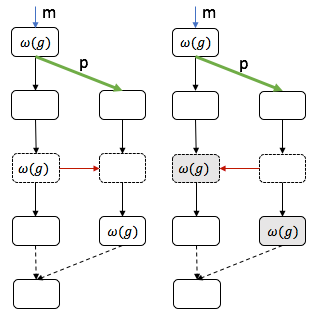
\includegraphics[scale=0.7]{../figs/example-cg}
  \caption{Two computation graphs for the program in \figref{fig:example}: the schedule on the left has no data-race and while the right does.}
%  \vspace{-2em}
   \label{fig:example-cg}
   \end{center}
\end{figure}

